\chapter{Numerische Ergebnisse}

In diesem Kapitel werden wir mit unserer persönlichen Implementierung das \enquote{Hadeler Problem}

\begin{gather*}
    T(z) = (e^z - 1) B_1 + z^2 B_2 - B_0 \\
    B_0 = b_0 I_n,
    \quad
    B_1 = (b_{j k}^{(1)}),
    \quad
    B_2 = (b_{j k}^{(2)}) \\
    b_{j k}^{(1)} = (n + 1 - \max(j, k)) j k,
    \quad
    b_{j k}^{(2)} = n \delta_{j k} + 1 / (j + k),
    \quad
    j, k = 1, \dots, n,
\end{gather*}

aus \cite{saad2020rational} lösen, und die theoretischen Ergebnisse veranschaulichen.

Wir legen die Parameter mit $n = 200$, $b_0 = 100$ fest und wählen unsere Kurve als Kreis mit Mittelpunkt $\texttt{z} = -30$ und Radius $\texttt{R} = 11.5$.
Als Toleranz zur Bestimmung der \enquote{korrekten} Singulärwerte wählen wir $\texttt{tol} = 10^{-5}$.

Im ersten Testlauf plotten wir die berechneten Eigenwerte im Vergleich zu den zusätzlich aussortierten Werten.
Zur besseren Veranschaulichung haben wir die Quadraturpunkte, über die wir summieren, auch miteingezeichnet.
Wie man in Abbildung \ref{fig:plot1} sieht, befinden sich die, von unserem Algorithmus als \enquote{korrekt} identifizierten, Eigenwerte alle innerhalb unserer Konturintegralkurve, während die zusätzlichen Werte außerhalb liegen.

\begin{figure}[H]
  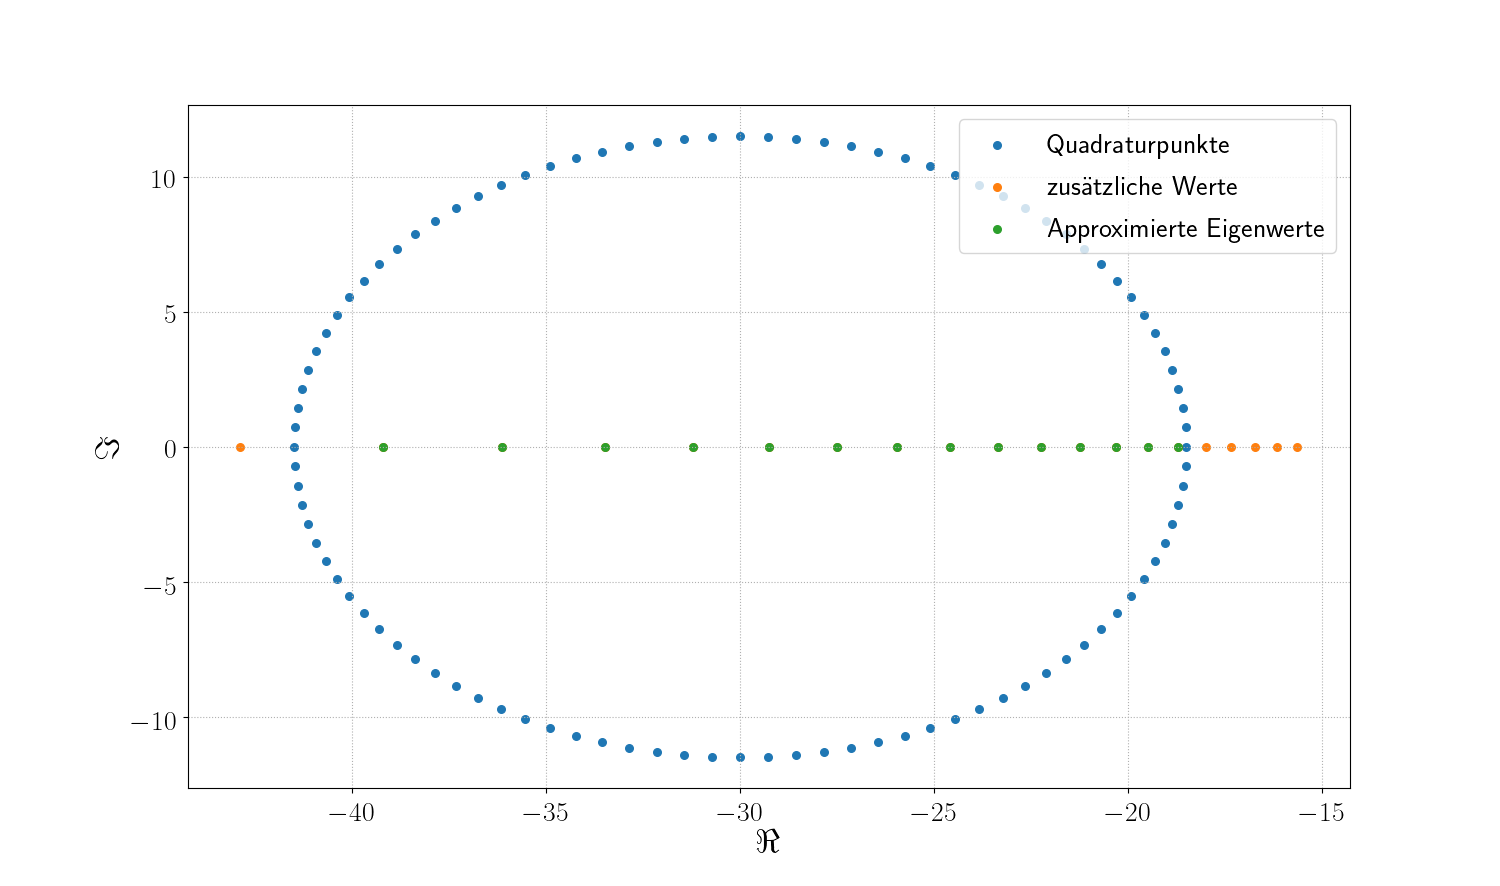
\includegraphics[width = \linewidth]{Plots/eigenwerte_complex_plot.png}
  \caption{Approximierte Eigenwerte vs. zusätzliche Werte}
  \label{fig:plot1}
\end{figure}

\section{Cut-Off}

In Abbildung \ref{fig:plot2} sehen wir den Vergleich der Größenordnungen der eigentlichen Singulärwerte mit den zusätzlichen Singulärwerten.
Nachdem hier ein deutlicher Abfall zu erkennen ist, ist es nicht schwer, die zusätzlichen Werte auszusortieren.

\begin{figure}[H]
  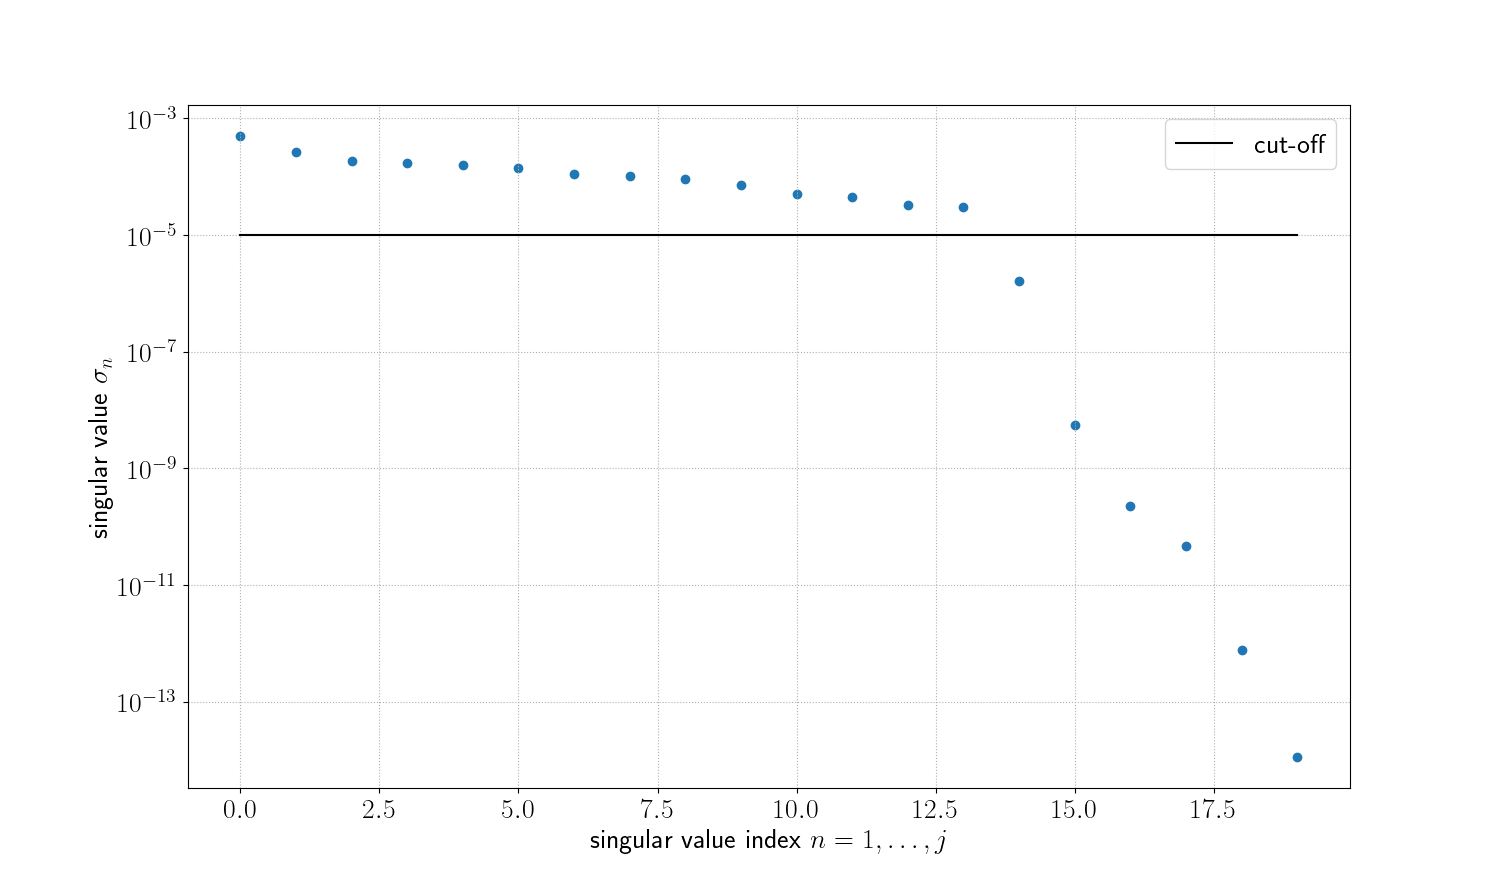
\includegraphics[width = \linewidth]{Plots/singulaerwerte_plot.png}
  \caption{Echte vs. zusätzliche Singulärwerte}
  \label{fig:plot2}
\end{figure}

Eine Heuristik zur Überprüfung der Qualität eines approximierten Eigenwerts $\lambda$ besteht darin, die Konditionszahl der jeweiligen Matrix $A(\lambda)$ zu betrachten.
Da wir gegen eine singuläre Matrix konvergieren sollten, würden wir erwarten, dass die Konditionszahl gegen unendlich geht.
In der Tat ist das Fall und man erkennt in Abbildung \ref{fig:plot3} sogar einen deutlichen Unterschied zwischen den echten und zusätzlichen Eigenwerten.

\begin{figure}[H]
  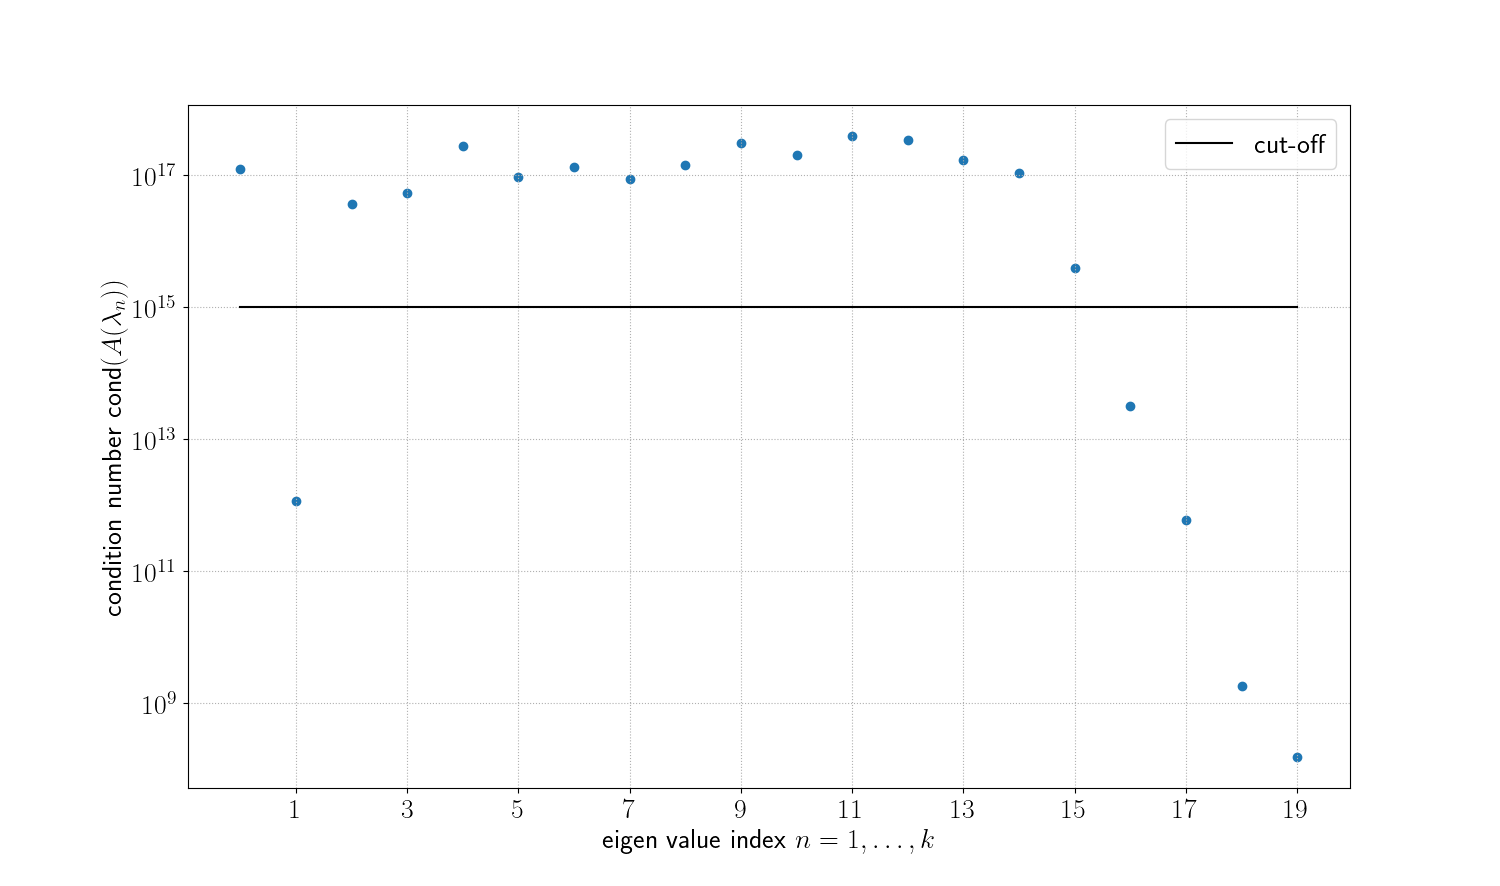
\includegraphics[width = \linewidth]{Plots/conditionnumber.png}
  \caption{Konditionszahlen von $A(\lambda_n)$}
  \label{fig:plot3}
\end{figure}

\section{Pitfalls}

Schlussendlich wollen wir noch Situationen aufzeigen, an denen der Algorithmus scheitert.
Die erste Möglichkeit dafür besteht darin, dass die Quadratur zu ungenau ist, und somit die \blockquote{korrekten} Singulärwerte nicht mehr von den zusätzlichen Werten zu unterscheiden sind.
In Abbildung \ref{fig:plot4} sieht man, wie sich die approximierten Singulärwerte bei unterschiedlicher Anzahl von Quadraturknoten verhalten.
Ab $\texttt{m} \geq 20$ Quadraturknoten aufwärts ist bereits ein Sprung zwischen den echten und zusätzlichen Werten zu erkennen, der sich bei steigender Anzahl noch verdeutlicht.

\begin{figure}[H]
  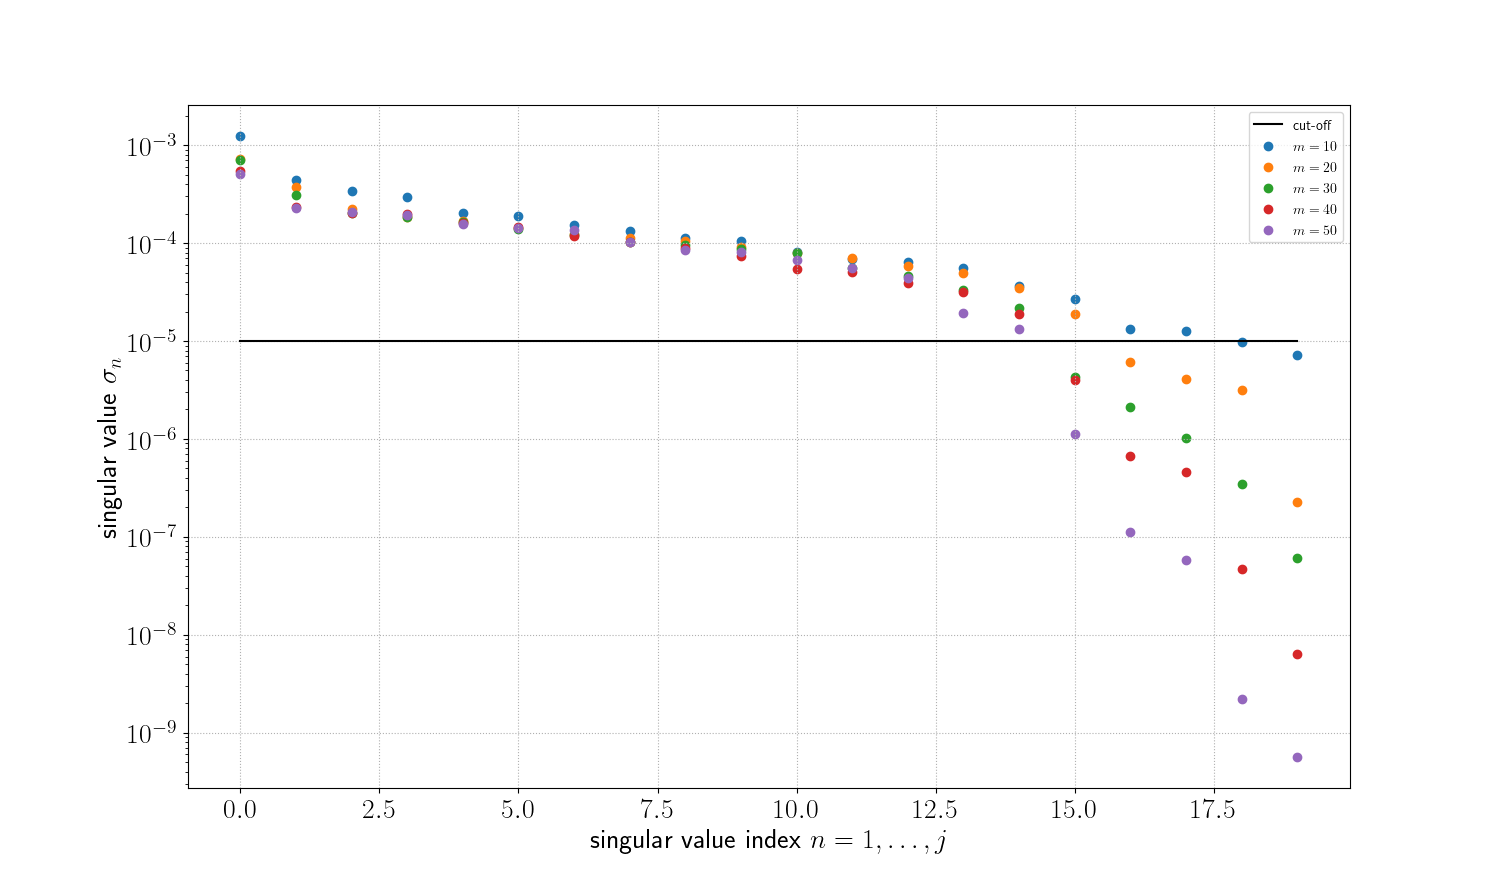
\includegraphics[width = \linewidth]{Plots/singulaerwerte_quadraturknoten.png}
  \caption{Singulärwerte in Abhängigkeit von der Anzahl der Quadraturknoten}
  \label{fig:plot4}
\end{figure}

Das zweite Hauptproblem ist, wenn die Zufallsmatrix zu klein gewählt wird.
Sollte die Zufallsmatrix weniger Spalten haben, als wir Eigenwerte innerhalb unserer Kurve erwarten, könnte man ja noch hoffen, zumindest einen Teil der Eigenwerte korrekt approximieren zu können.
Wie man in Abbildung \ref{fig:plot5} sieht, können wir in der Regel nicht einmal das erwarten.

\begin{figure}[H]
  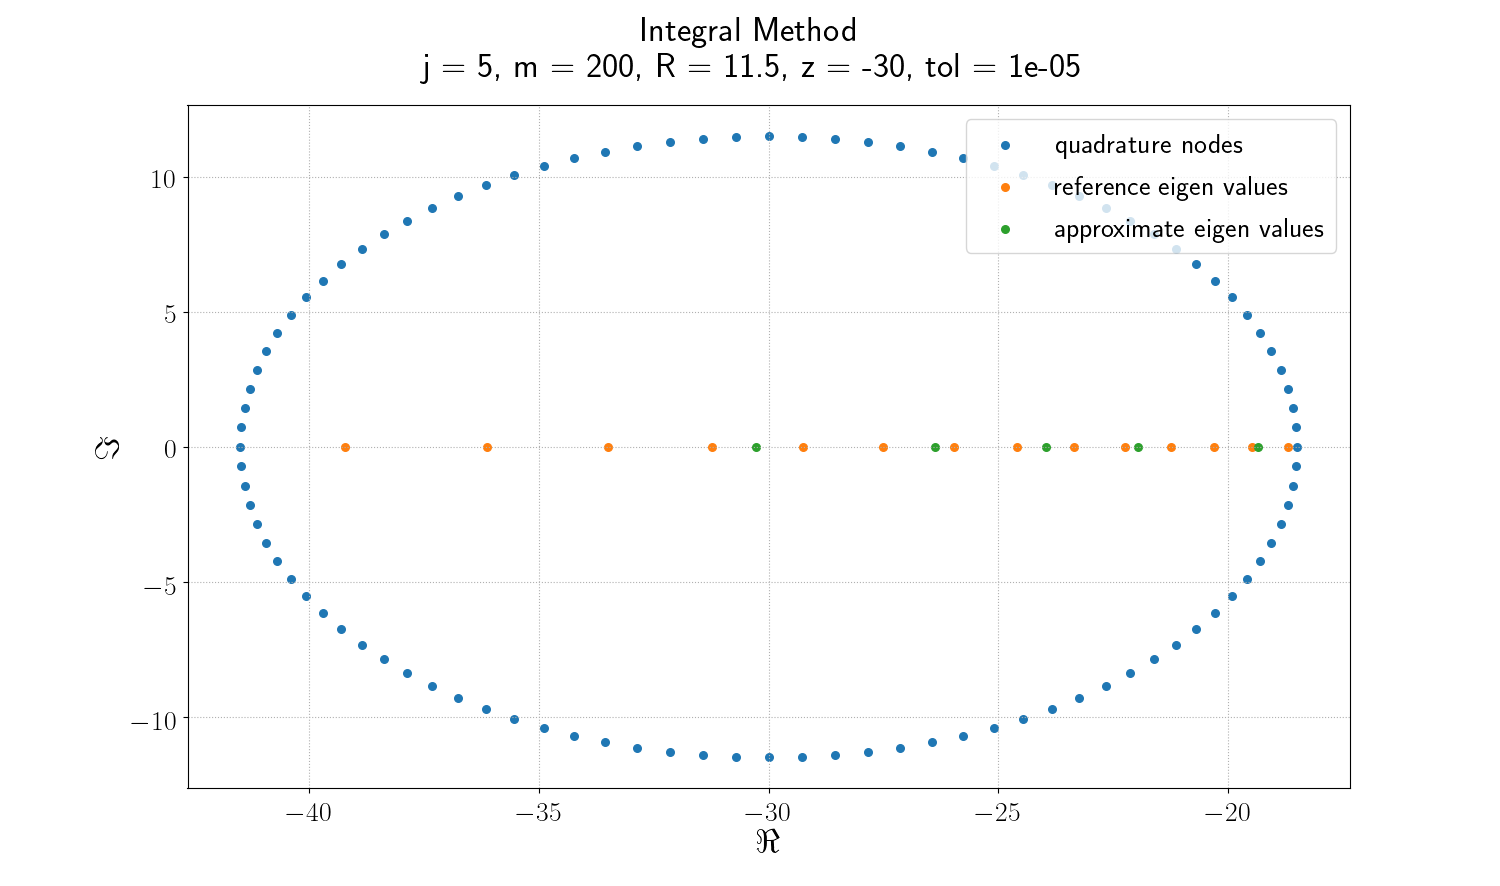
\includegraphics[width = \linewidth]{Plots/zufallsmatrix_zu_klein.png}
  \caption{Zu kleine Zufallsmatrix}
  \label{fig:plot5}
\end{figure}

